\documentclass[a4paper,11pt]{article}
\pdfmapfile{=tengwarscript.map}
\usepackage[T1]{fontenc}
\usepackage[utf8]{inputenc}
\usepackage{lmodern}
\usepackage[french]{babel}
\usepackage[squaren, Gray]{SIunits}
\usepackage{circuitikz}
\usepackage{graphicx}
\usepackage{amsmath}
\usepackage{amssymb}
\usepackage{mathrsfs}
%\usepackage{subfigure}
\usepackage[absolute]{textpos}
\usepackage{url} 
\usepackage[toc]{appendix}
\usepackage{array}
\usepackage[final]{pdfpages}
\usepackage{listings}
\usepackage[Lenny]{fncychap}
\usepackage{multirow}
\usepackage{ragged2e}
\usepackage{verbatim}
\usepackage[top=2cm, bottom=2cm, left=2cm, right=2cm]{geometry}
\usepackage[rightcaption]{sidecap}
%\usepackage{systeme}
\usepackage{listings}
\usepackage{courier}
\usepackage{color}
\usepackage{here}
\usepackage{caption}
\usepackage{subcaption}
\usepackage[annataritalic]{tengwarscript}
\providecommand{\e}[1]{\ensuremath{\times 10^{#1}}}

%%%%%%%%%%%%%%%%
%						%
%	Listing code Matlab		%
%						%
%%%%%%%%%%%%%%%%

\usepackage{listingsutf8}
\usepackage{color}
\renewcommand{\lstlistingname}{Code}
\usepackage{textcomp}
\definecolor{listinggray}{gray}{0.9}
\definecolor{lbcolor}{rgb}{0.9,0.9,0.9}
\lstset{
	backgroundcolor=\color{lbcolor},
	numbers=left,
	tabsize=4,
	rulecolor=,
	language=matlab,
        basicstyle=\scriptsize,
        upquote=true,
        aboveskip={1.5\baselineskip},
        columns=fixed,
        showstringspaces=false,
        extendedchars=false,
        inputencoding=utf8/latin1,
        breaklines=true,
        prebreak = \raisebox{0ex}[0ex][0ex]{\ensuremath{\hookleftarrow}},
        frame=single,
        showtabs=false,
        showspaces=false,
        showstringspaces=false,
        identifierstyle=\ttfamily,
        keywordstyle=\color[rgb]{0,0,1},
        commentstyle=\color[rgb]{0.133,0.545,0.133},
        stringstyle=\color[rgb]{0.627,0.126,0.941},
}


\newcommand{\HRule}{\rule{\linewidth}{0.5mm}}

\begin{document}

\begin{titlepage}

  \begin{center}

% Upper part of the page

    \textsc{\Large Université Catholique de Louvain}\\[0.5cm]

    \textsc{\LARGE{ Projet en Elements Finis}}\\[0.2cm]


% Title
    \HRule \\[0.2cm]
    {\huge \bfseries Modéliser le tsunami du Japon}\\ % TODO change
    \HRule \\[0.2cm]

    \HRule \\[0.2cm]
        \end{center}
      \begin{figure}[h!]
      \begin{center}
      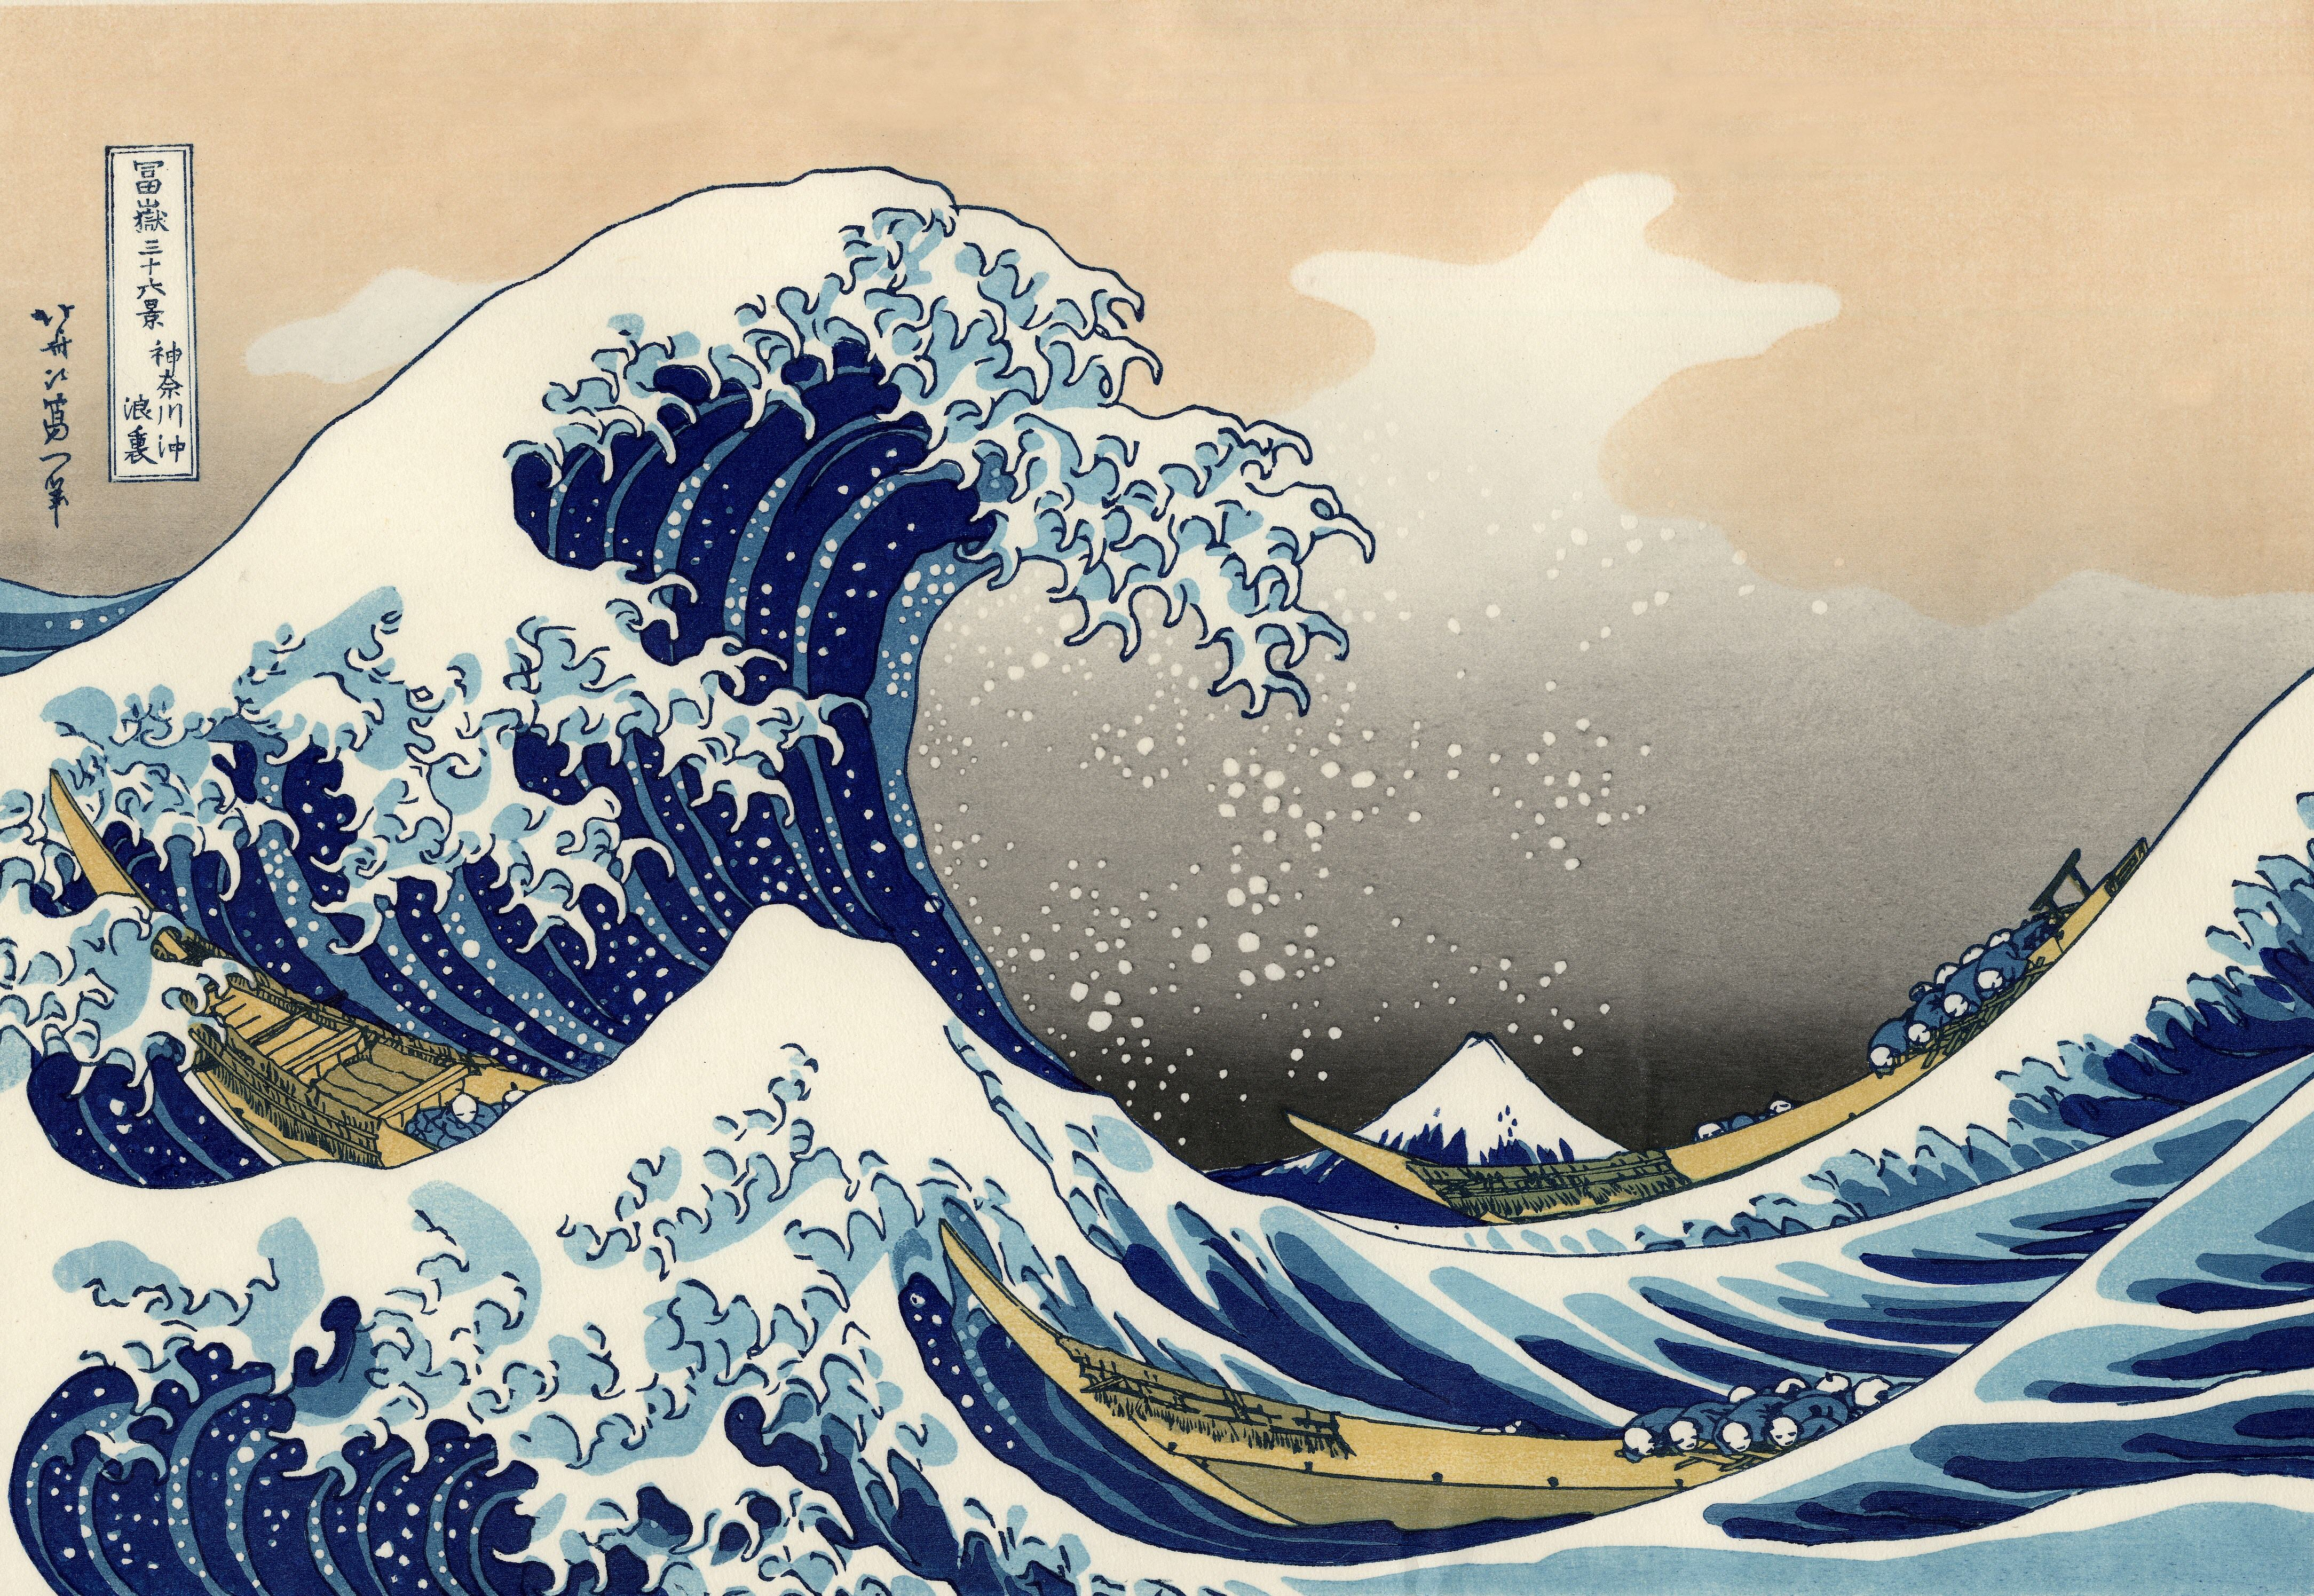
\includegraphics[width=14cm]{BigWave.jpg}
      \end{center}
      \end{figure}

    \begin{center}
    \HRule \\[0.2cm]
  \end{center}

    \begin{minipage}{0.48\textwidth}
      \begin{flushleft} \large
        \textit{Auteurs:}\\
        Laurent \textsc{Debersaques } (NOMA BITCH!)\\
        Maxime \textsc{De Mol} (21941100)\\

      \end{flushleft}
    \end{minipage}
    \begin{minipage}{0.48\textwidth}
      \begin{flushright} \large
        \textit{Cours:} \\
        MECA1120\\ \vspace{0.27cm}
       
        \textit{Professeurs:} \\
        Vincent \textsc{Legat}\\ \vspace{0.9cm}
        
        \textit{Groupe:} \\
        10
      \end{flushright}
    \end{minipage}

    \vfill
% Bottom of the page

    \begin{minipage}{0.3\textwidth}
      \begin{flushleft}
        
\includegraphics[height=2cm]{logo_UCL.jpeg}
      \end{flushleft}
    \end{minipage}
    \begin{minipage}{0.3\textwidth}
      \begin{center}
        %{\large FSA12BA}\\
        {\large \today}
      \end{center}
    \end{minipage}
    \begin{minipage}{0.3\textwidth}
      \begin{flushright}
        
\includegraphics[height=2cm]{logo_EPL.png}
      \end{flushright}
    \end{minipage}
\end{titlepage}


\tableofcontents
%\newpage

\vspace{10mm}
\textit{A l'attention du Service d'Océanographie.}\\

Il y a quelques jours il nous a été demandé de réaliser une modélisation du tsunami ayant dévasté le Japon en 2011. Cette brève note explicative a pour but de vous familiariser avec la précision de la méthode utilisée. Nous réaliserons également une analyse de l'erreur de notre modèle ainsi qu'une comparaison avec le résultat d'autres études, indépendantes de la notre. Finalement, nous décrirons les mesures prises pour rendre le code de calcul plus rapide et terminerons par une présentation de l'interface graphique.\\

\section{Estimation de l'ordre de précision}
\label{sec:error}

Pour vous fournir une estimation la plus proche possible de la réalité nous utilisons la méthode des éléments finis, qui est très largement utilisée de par son son efficacité et sa précision \cite{FEM}. Cette discipline fait appel à des méthodes numériques, une branche dans laquelle il faut toujours s'intéresser à l'ordre de précision de la méthode en question. Dans notre contexte, une estimation de cette erreur est possible à partir des résultats obtenus sur différents maillages d'éléments, qui diffèrent entre eux au niveau de leur finesse, comme l'illustre la figure \ref{fig:mesh}.\\

\begin{figure}[H]
        \centering
        \begin{subfigure}[b]{0.3\textwidth}
                \centering
                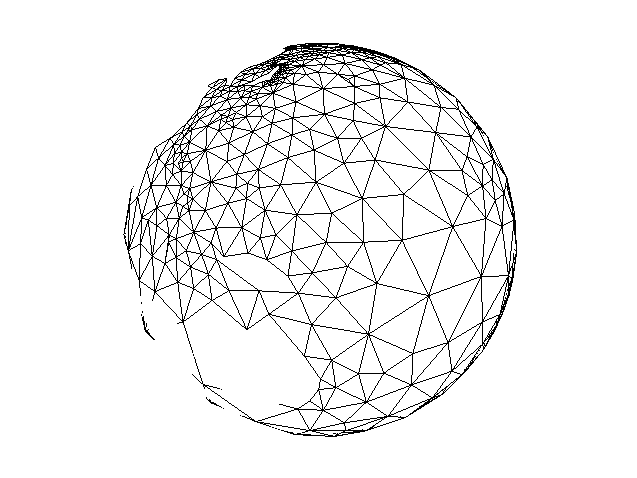
\includegraphics[width=\textwidth]{TriTiny.png}
                \caption{Grossier}
                \label{fig:tiny}
        \end{subfigure}
        %\quad
        \begin{subfigure}[b]{0.3\textwidth}
                \centering
                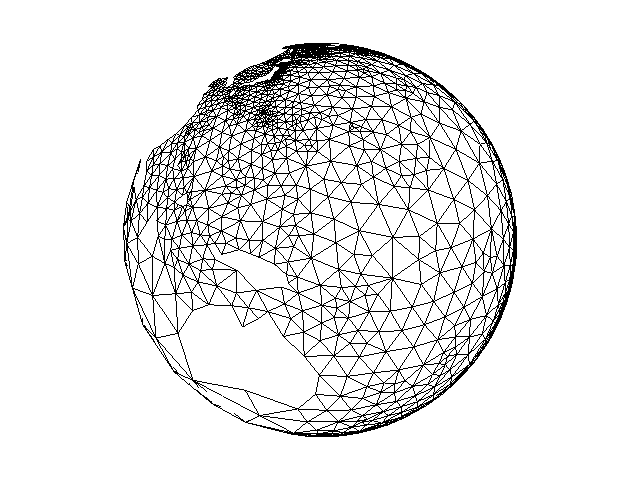
\includegraphics[width=\textwidth]{TriSmall.png}
                \caption{Petit}
                \label{fig:small}
        \end{subfigure}
       % \quad
        \begin{subfigure}[b]{0.3\textwidth}
                \centering
                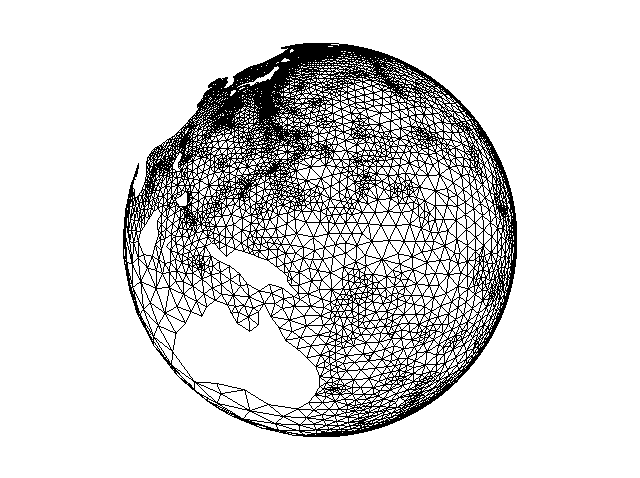
\includegraphics[width=\textwidth]{TriMedium.png}
                \caption{Moyen}
                \label{fig:medium}
        \end{subfigure}
        \caption{Exemple de différents maillages d'éléments triangulaires}\label{fig:mesh}
\end{figure}

Plus le maillage est fin, meilleurs seront les résultats (du point de vu de la précision). Pour pouvoir comparer nos résultats, nous utilisons comme référence la simulation sur le maillage le plus fin à notre disposition (davantage encore que celui en \ref{fig:medium}), et comparerons le niveau d'élévation de l'océan $\eta$, obtenus sur les maillages en question. Suite à la différence de topologie entre les maillages, nous nous servirons de la moyenne de cette élévation, $\overline{\eta}$, définie comme:

\begin{equation}
|\overline{\eta}| = \dfrac{\sum\limits^{n_{nodes}}_{i=1} |\eta_i|}{n_{nodes}}
\end{equation}

Avec la moyenne de l'élévation de référence, c'est à dire à partir de la solution calculée sur notre maillage le plus fin, à l'ordre le plus élevé\footnote{Il s'agit d'un maillage de quadrilatère comptant quelque 70 000 noeuds}, $\overline{\eta_r}$, nous pouvons définir l'erreur comme étant:

\begin{equation}
e = ||\overline{\eta_r}|-|\overline{\eta}||
\end{equation}

Nous définissions le pas $h$ comme étant la racine carrée de la moyenne des surfaces des éléments de nos maillages.\\
\begin{table}
\centering
\begin{tabular}{| l || c | c || c |}
\hline
Maillage & $e$ lin & $e$ quad & $h\hspace{1mm}[m]$\\
\hline \hline
\multicolumn{4}{|c|}{Triangles} \\
\hline \hline
Tiny & 0.0021 & 7.46\e{-4} & 1.307\e{6} \\
\hline
Small & 4.79\e{-4} & 1.49\e{-4}& 7.745\e{5}\\
\hline
Medium & 2.72\e{-4} & 2.02\e{-5} & 3.166\e{5} \\
\hline \hline
\multicolumn{4}{|c|}{Quadrilatères} \\
\hline \hline
Tiny & -9.7\e{-4} & 7.17\e{-4} & 5.304\e{5}\\
\hline
Small & 0.0011 & & 3.146\e{5}\\
\hline
Medium & 6.19\e{-5} & & 1.286\e{5}\\
\hline
\end{tabular}
\caption{Erreurs en fonctions du maillage}
\label{tab:err}
\end{table}

Grâce aux mesures expérimentales reprises dans le tableau \ref{tab:err}, nous allons pouvoir approcher l'ordre de de précision réel en recherchant le terme de proportionnalité $O(h^x)$ de l'erreur\footnote{$O(h^x)$ veut dire que l'erreur est proportionnelle à $h$, et que si $h$ est réduit de moitié, l'erreur va diminuer d'un facteur $2^x$}, $x$ étant dès lors notre ordre de précision.\\

On obtient, après calcul, un ordre de 2 pour les éléments (bi)linéaires et un ordre de 3 pour les éléments (bi)quadratiques. En effet, à titre d'exemple, on peut remarquer que entre le maillage Tiny\footnote{Figure \ref{fig:tiny}} et Small\footnote{Figure \ref{fig:small}}, le h moyen est divisé par un facteur 2 alors que l'erreur se retrouve divisée par 4, ce qui correspond bien à un facteur $O(h^2)$.

\section{Validation}

L'ordre de précision seul ne permet pas de juger de la qualité d'une simulation. C'est pour cela que nous comparons nos résultats avec une autre étude, celle de la NOAA\cite{NOAA}, qui retrace le parcours réel du tsunami. On peut voir sur la figure \ref{fig:noaa} que la vague principale atteints les côtes de la Papouasie 6h après le séisme.\\
Sur notre modélisation, après 12000 itérations avec un pas de temps de 2 secondes entre chaque itération, ce qui nous amène à une simulation du vague pour 6h40min, nous obtenons la figure \ref{fig:cote}.\\

L'analogie entre ces 2 images nous permet de de juger notre simulation assez proche de la réalité, et donc fiable pour la prédiction d'un tsunami.

\begin{figure}[H]
\centering
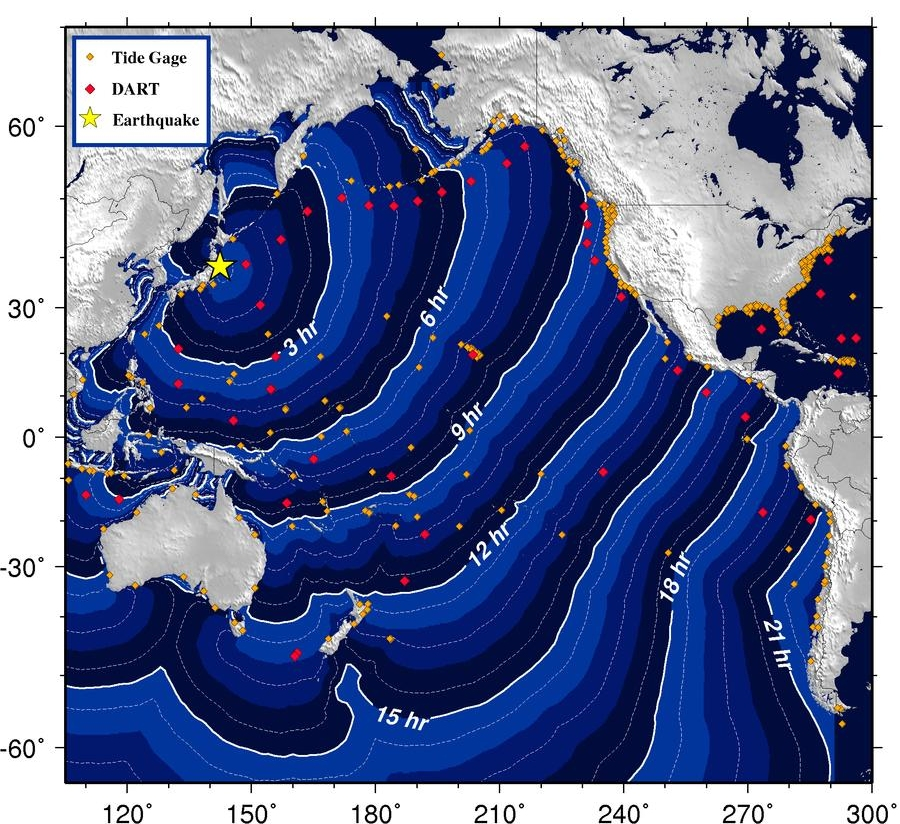
\includegraphics[width=0.7\linewidth]{NOAA.jpg}
\caption{Evolution du tsunami du Japon}
\label{fig:noaa}
\end{figure}

\begin{figure}[H]
\centering
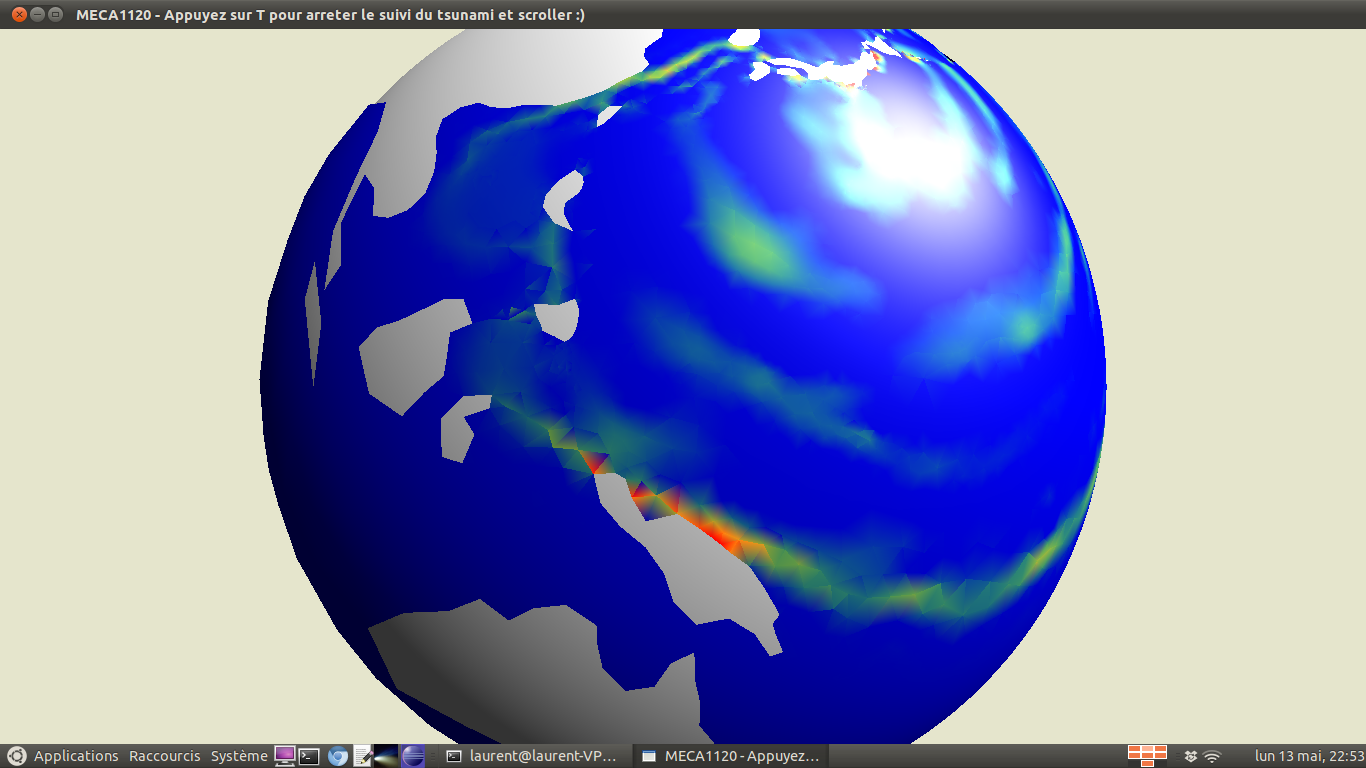
\includegraphics[width=0.8\linewidth]{Cotes.png}
\caption{Simulation 6h40 après le seisme}
\label{fig:cote}
\end{figure}


\section{Optimisation du code}

Comme expliqué dans la section \ref{sec:error}, affiner le maillage permet un gain de précision. Mais ce gain vient au prix d'un coup calcul plus élevé, dû au nombre de noeuds revu à la hausse, ce qui se traduit par un temps de simulation (nettement) plus long. Optimiser notre code, au sens de la vitesse, est donc un point important. Pour cela, plusieurs solution ont été implémentées dans notre modélisation.\\

\subsection{Diviser pour mieux régner}

Si l'utilisateur n'indique pas clairement lors de la conception de son programme qu'il veut utiliser plusieurs unités de calcul (dit core) en même temps pour son logiciel, celui ci ne s'exécute que sur un core à la fois. Une grosse perte de temps et de ressources quand on sait que la plupart des systèmes actuels sont équipés de processeur multicores. Répartir les calculs sur plusieurs fils d'exécution permet un gain de temps considérable, à condition que les calculs à exécutés soient parallélisables.\\

Dans le cas de notre simulation du tsunami, nous avons su multithreader (rendre parallèle) le calcul de certaines intégrales. Le code entier est loin d'être complètement parallèle, mais nous avons su augmenter les performances d'environ 80\% en utilisant 4 coeurs.\\

\subsection{Eviter le travail inutile}

Dans la méthode des éléments finis, il existe certaines variables qui restent inchangées pour un élément donné au fil des itérations successifs. Il est dés lors bête de consommer des ressources processeur en recalculant ces variables. La solution adoptée dans notre programme est de précalculer toutes ces valeurs avant le début de la simulation, de les stocker dans des vecteurs, et de les mettre à disposition des fonctions de calcul, ce qui exclut le recalcul inutile de celles-ci.

\section{Interface graphique}

L'interface graphique a été modifiée par nos bon soins afin de satisfaire les envies diverses que pourrait avoir l'utilisateur de notre programme ! Elle comporte en effet deux modes :\\

\begin{itemize}
 \item \textbf{Le mode automatique}. Il est sélectionné par défaut au lancement du programme. La caméra se positionne de sorte à suivre automatiquement le tsunami et s'arrange pour l'afficher au mieux.\\
  \item \textbf{Le mode libre}. La caméra ne bouge plus automatiquement et c'est désormais l'utilisateur qui est aux commandes ! Il aura la possibilité de scroller avec la molette de sa souris afin de (dé)zoomer sur la terre. Il pourra également maintenir le clic gauche enfoncé tout en glissant la souris de sorte à faire tourner le globe.\\
\end{itemize}

A tout instant, il est possible de passer d'un mode à l'autre en appuyant sur la touche \texttt{T} du clavier. Attention cependant, la détection du clavier est assez sensible et il ne faut pas maintenir la touche enfoncée trop longtemps :)



\bibliographystyle{plain}
%\nocite{*}
\bibliography{bibliographie.bib}


\vfill
\begin{center}
\tengwarannataritalic[0.75]
\tengwa{254}
\Textendedcalma\TTthreedots\Tnuumen\Tessenuquerna\TTthreedots\Tungwe\Tando\Toore\TTrightcurl\Tumbar\Ttinco\TTthreedots\Tlambealt\TTrightcurl\Tquesse\TTdoublerightcurl
\Tromanperiod\Ts
\Textendedcalma\TTthreedots\Tnuumen\Tessenuquerna\TTthreedots\Tungwe\Tungwe\Tumbar\TTnasalizer\TTdot\Ttinco\TTthreedots\Tlambe\TTrightcurl
\tengwa{255}\\
\Textendedcalma\TTthreedots\Tnuumen\Tessenuquerna\TTthreedots\Tungwe\Tthuule\Troomen\Tquesse\TTthreedots\Ttinco\TTthreedots\Tlambealt\TTrightcurl\Tquesse\TTdoublerightcurl
\Tromanperiod\Ts
\Textendedungwe\TTthreedots\Tumbar\Toore\TTrightcurl\Tesse\Tkern{-0.2}\Tmalta\TTrightcurl\Textendedcalma\TTdot\Ttelco\TTdot\Tquesse\Troomen\Tparma\TTnasalizer\TTdot\Ttinco\TTthreedots\Tlambe\TTrightcurl
\end{center}

\end{document}